\chapter{Praktická část}
V praktické části se tato práce zaměřuje především na porovnání výkonu klasických SQL databází s novými NoSQL databázemi. Nelze však porovnávat kteroukoliv NoSQL databázi s kteroukoli SQL databází, protože většina NoSQL řešení je navržena k provozu v zcela jiných oblastech webové aplikace, než se používají běžné SQL servery. Proto byly z těchto dvou přístupů vybráni dva zástupci, kteří se zpravidla používají ke stejnému účelu, tedy perzistentnímu ukládání dat\footnote{Trvalé úkládání důležitých (například uživatelských) dat.} webové aplikace.

Těmito zástupci jsou MongoDB ze světa NoSQL databází a MySQL ze světa SQL databází. Obě databázová řešení jsou postavena na podobných konceptech, dokumentace MongoDB dokonce přímo porovnává možnosti a syntaxi s SQL servery \cite{mongoMySQLMapChart}.
Databáze budou porovnány z hlediska výkonu základních operací, především rychlosti uložení a následného získání dat. Testy budou spouštěny paralelně ve více instancích zároveň, budou se snažit simulovat reálnou konkurenci připojených klientů, která je u dnešních webových aplikací běžná. 

Jednotlivé databázové servery byly provozovány lokálně kvůli relevantním výsledkům testů, které tak nebudou náchylné na problémy nebo případné výpadky připojení. Na základě provedeného měření bude rozhodnuto, zda-li je NoSQL databáze MongoDB opravdu rychlejší než MySQL a jaký přínos v rychlosti bude mít databázový cluster. Veškeré ukázky příkazů a kódu v práci jsou zaměřeny na UNIXové systémy, mohou však fungovat i na platformě Windows s určitými změnami. Mezi těmito dvěma platformami je velký rozdíl především v adresářové struktuře.
\section{Vybraná databázová řešení}
Jako nejvhodnější kandidát pro porovnávání s SQL databázemi, byla vybrána dokumentově orientovaná databáze MongoDB. Hlavním důvodem tohoto výběru je velmi podobné zaměření NoSQL databáze MongoDB. I když se v principu stále jedná o key-value databází, jednotlivé objekty databáze vystupují jako logické celky (kolekce), na které lze nahlížet analogicky jako na SQL tabulky. Databáze MongoDB dokáže sloužit pro ukládání prakticky jakýchkoliv dat, je ale často nasazována u webových aplikací jako přímá náhrada SQL serverů.

Ze světa SQL databází byla vybraná asi nejpoužívanější open source databáze MySQL, které je mezi vývojáři webových aplikací velmi oblíbená hlavně kvůli jednoduchosti nasazení a její obsluhy. Existuje velké množství frameworků a knihoven, které zjednodušují práci s SQL serverem. Tyto knihovny se snaží objektový přístup, používaný v logice aplikace, převést na relační přístup, který používá SQL databáze. Dokumentově orientované NoSQL databáze jako je MongoDB takové nástroje nepotřebují, slouží totiž přímo jako objektové úložiště.

\section{Metodika měření a očekávané výsledky}
Obě databáze budou porovnány z hlediska rychlosti zpracování databázových operací. Porovnávány budou časové úseky, které databázový server nebo cluster potřebuje na zpracování požadavku. Těmito požadavky bude například vložení velkého počtu dat najednou a jejich následné získání podle klíče nebo jiné podmínky. Získaná množina dat bude ještě zobrazena, tím pádem dojde k skutečnému získání celé vybrané množiny z databáze. Tento mechanismus je nutné doplnit proto, že databázové ovladače optimalizují práci s databází a většinou vrací pouze iterátor, přes který je nutné postupně získat a zobrazit získaná data po jednom řádku. Iterátor je návrhový vzor, který obsahuje data vždy právě jednoho řádku tabulky a umožňuje procházet prvky zpravidla pomocí metod \emph{next()} a \emph{previous()}. Často se používá jako obalovací objekt pro výsledek databázového dotazu. Tato operace se většinou nazývá \emph{SELECT + FETCH}.

Dále bude testována operace přidání indexu nad množinu dat, která je u obou databází velmi náročná. Práce s indexy navíc zablokuje databázové servery, které nemohou po dobu provádění příkazu, zpracovávat další požadavky. Doba zpracování indexační operace je závislá na velikosti dat, které jsou v kolekci uloženy, proto je velmi vhodné rozmyslet si indexy již při návrhu databáze, nicméně MongoDB by mělo i v tomto ohledu dosahovat vyšších rychlostí než MySQL. Poslední operací, která bude nad databázemi testována, je smazání jednoho nebo více záznamů.

Testovací prostředí je napsané v programovacím jazyce PHP. Měření probíhá pomocí porovnání systémového času serveru před provedenou operací a po ní pomocí PHP funkce \emph{microtime()}, která vrací UNIXový timestamp. \footnote{Počet sekund od 1.1.1970 00:00:00.}

\begin{lstlisting}[caption={Ukázka kódu provádějícího měření}]
$t=microtime(true);
doSomething();
$result=microtime(true)-$t;
\end{lstlisting}

Přesnost uvažovaného postupu měření je dostatečná, jak dokládá provedený test doby běhu funkce \emph{sleep(3)}, která na zadanou dobu uspí provádění programu. Tato operace, podle provedeného měření, trvala 3.0008780956268 sekundy. Prostředí pracuje s velkou množinou náhodně vygenerovaných dat, které nejdříve načte do paměti a poté s nimi dále pracuje. Kvůli velikosti testovacích dat je také nutné zvýšit maximální velikost paměti, kterou může PHP alokovat.

Testovací prostředí přistupuje k databázím pomocí tzv. databázových ovladačů. Tyto ovladače představují sadu tříd, sloužících k obsluze databázového serveru. Pro přístup k MongoDB se používá ovladač MongoClient, který je volně dostupný jako rozšíření do PHP a poskytuje všechny možnosti práce s databází. Rozšíření obsahuje třídy MongoClient, MongoDB, MongoCollection a MongoCursor, z nichž každá reprezentuje určitou část MongoDB databáze. Třída MongoCursor je obalující třída (iterátor), obsahující samotná data získaná z  databáze. Modul pro práci s MongoDB není standardní součástí PHP a je nutné jej doinstalovat. Na UNIXových systémech je instalace jednoduchá pomocí nástroje \emph{pecl}. Na Windows existují zkompilované DLL knihovny, které je třeba ručně přidat do konfigurace PHP pomocí příkazu \emph{extension} \cite{phpMongo}. 

\begin{lstlisting}[caption={Instalace MongoDB rozšíření do PHP na UNIXových systémech}]
sudo pecl install mongo
\end{lstlisting}
Obsluha standalone MongoDB databázového serveru se nijak neliší od obsluhy databázového clusteru, je tedy doporučováno začít s aplikací na jednom serveru a v případě úspěchu aplikace a tím pádem větší zátěže generované uživateli, nasadit MongoDB cluster.

Operace nad MySQL serverem budou realizovaný pomocí knihovny NotORM Jakuba Vrány, která poskytuje jednoduché rozhraní pro práci s MySQL databázovým serverem. Knihovna poskytuje třídy reprezentující jednotlivé části databáze a nabízí široké možnosti dotazování. Jedná se o tenkou knihovnu, pouze zjednodušující práci s SQL serverem tím, že automaticky generuje SQL dotazy. Vzhledem k jednoduchosti knihovny lze říci, že její použití nebude mít žádný nebo minimální vliv na výsledky provedených testů \cite{notOrm}. 

Výsledkem provedených testů budou časové údaje stejných operací se stejnými daty provedených nad SQL databází MySQL a NoSQL databází MongoDB. Tyto databáze budou spouštěny jako standalone servery, tedy v režimu kdy jeden server obstará veškerou obsluhu databáze. Testy budou poté pro doplnění spuštěny také na MongoDB databázovém clusteru. Každý test bude spuštěn paralelně pětkrát, výsledné časy testů budou vytvořeny prostým aritmetickým průměrem.
Lze předpokládat, že na testované konfiguraci bude nejrychlejší MongoDB standalone server, síla clusteru se projeví až při skutečném nasazení na fyzické servery a při velmi vysoké zátěži.

\section{Testovací data}
Testovacími daty této práce budou objekty reprezentující fiktivní uživatele nějaké společnosti.
Jedná se o vysoce strukturované data, obsahující většinu datových typů (řetězec, celé číslo, desetinné číslo, logická hodnota, datum, čas, pole apod.). Zároveň je v nich realizována většina vazeb, které musejí být u relačních databází řešeny dalšími tabulkami. Bylo vytvořeno několik SQL tabulek a několik tříd aplikační logiky v PHP pro účely tohoto testovaní. Do NoSQL databáze MongoDB je možné tyto objekty ukládat přímo.

\begin{lstlisting}[caption={Ukázka objektu testovacích dat (zkráceno)}]
  {
    "hash": "53e0b94367d25cf04192f656",
    "index": 0,
	...
    "email": "rosannewhitfield@medcom.com",
    "phone": "+1 (906) 497-3016",
    "address": "611 Ovington Court, Curtice, New York, 6257",
    "registered": "2014-05-30T05:04:03 -02:00",
    "latitude": 49.332297,
    "longitude": -131.785071,
    "tags": ["do",
	  ...
    ],
    "friends": [
      { "id": 0,
        "name": "Sonja Moses"
      },
	  ...
    ],
    "favoriteFruit": "banana"
  },
\end{lstlisting}
Soubor testovacích dat tvoří 4 sady náhodně generovaných objektů po 25 000 záznamech. Data jsou uložena ve formátu JSON. Testovací prostředí načítá jednotlivý dataset do paměti, pokud je třeba testovat více než 25000 objektů zároveň, lze pomocí příkazu \emph{nextDataset()} získat další dataset. Je tedy možné v testech pracovat až se 100 000 unikátními objekty. Objekty reprezentují fiktivní osoby zaměstnané v nějaké organizaci. Tyto objekty byly vygenerovány pomocí nástroje \emph{JSON - Generator}, který je volně dostupný na Internetu. Tento nástroj generuje JSON objekty podle zadaných kritérií, nebo vlastních funkcí napsaných v Javascriptu a výborně se hodí pro testovaní webových aplikací. 

\section{Testovací prostředí}
Výkonnostní testování databází bylo provedeno na osobním notebooku MacBook Air (mid 2013), který sice disponuje relativně nízkým výkonem, ale nabízí velmi rychlé SSD disky přimo napojené na sběrnici PCI Express. Díky velmi vysoké rychlosti diskových operací (až 700MB/s), lze v oblasti databází očekávat zajímavý výkon \cite{macDiskSpeed}. Jednoduchý MySQL server společně s jedním MongoDB serverem budou provozovány přímo v prostředí Mac OS X 10.9.2. Stejné testy byly provedeny i nad virtuálním MongoDB databázovým clusterem s 10 připojenými servery, spravovaným pomocí nástrojů Docker a VirtualBox v operačním systému Ubuntu.

Testovací prostředí je napsáno v PHP a testy se spouští pomocí obyčejného HTTP požadavku. V rámce lokálního Apache serveru běží PHP 5.4.21, které komunikuje s databázemi pomocí ovladačů. Podpora MySQL je dostupná v rámci rozšíření \emph{mysqli} 5.0.10, MongoDB  doplňuje \emph{mongo} extension ve verzi 1.4.5. Samotné testy jsou obyčejné PHP třídy, rozšiřující základního předka \emph{BPTestCase}, který přináší funkcionalitu měření. Každá z testovacích tříd je zaměřená na jiný typ databází, jednotlivé testy jsou v nich implementovány jako metody. Kvůli velkému objemu testovacích dat a časové náročnosti provedených testů, je třeba zvýšit maximální množství paměti, kterou může testovací prostředí použít. Zároveň je nutné vypnout časový limit provádění PHP skriptů. Tyto změny lze provést v konfiguraci PHP, nebo přímo v kódu pomocí volání funkce \emph{ini\_set()}.

\begin{lstlisting}[caption={Nutná konfigurace PHP prostředí}]
ini_set('max_execution_time', 0);
ini_set('memory_limit', '1024M');
\end{lstlisting}

Každá testovací třída také může obsahovat metodu \emph{beforeTests()}, která je vždy zavolána před začátkem testování. Tato metoda většinou provádí připojení a autentizaci do databáze. Testovací prostředí podporuje i metodu \emph{afterTests()}, která bude zavolána vždy po skončení všech testů. Tato metoda není v testech využita, protože odpojení od databáze a úklid provádějí PHP databázové ovladače automaticky. 

\begin{lstlisting}[caption={Ukázka HTTP požadavku který spustí test "insert1000Test" na třídě MongoTest}]
http://<url>/runner.php?class=MongoTest&test=insert1000Test
\end{lstlisting}

Testovací prostředí je spolu s testy dostupné na přiloženém CD.

\subsection{MySQL standalone server}
Prvním databázovým serverem testovaným v této práci byl MySQL server ve verzi 5.6.16. 
Databázový server MySQL je nejpoužívanější zdarma dostupnou variantou SQL serveru a druhou nejpoužívanější databází vůbec \cite{enginesRanking}. Tohoto umístění dosáhla díky jednoduchosti jejího nasazení, dobrému výkonu a především proto že se jedná o volně šiřitelnou databázi. Na rozdíl od komerčních řešení, MySQL dlouho nepodporovalo pohledy, triggery a uložené procedury. Tyto vlastnosti, spolu s mnoha dalšími, byly doplňeny až v posledních letech. Databázi vytvořila švédská společnost MySQL AB, později vlastněna firmou Sun Microsystems, která je dnes pod křídly Oraclu. Velmi často je nasazována jako hlavní databáze do webových PHP aplikací v kombinaci se servery Apache (tzv. LAMP \footnote{Linux, Apache, MySQL, PHP.}). MySQL server byl jeden z prvních produktů, který používal tzv. dvojí licencování. Databáze je totiž distribuována jednak pod svobodnou licencí GNU GPL v3, ale také pod placenou licencí zahrnující plnou podporu.

Server lze spustit ve formě daemonu \emph{mysqld} stejně jako MongoDB, ale častěji se spouští přímo v systému jako služba. Instalace je na linuxových systémech jednoduchá, například na Ubuntu a podobných systémem stačí stáhnout balíček \emph{mysql-server} \cite{mysqlUbuntu}. 
\begin{lstlisting}[caption={Instalace MySQL serveru na Ubuntu}]
sudo apt-get install mysql-server
\end{lstlisting} 
Příkaz výše nainstaluje MySQL server v Ubuntu a podobných linuxových systémech. Server pak lze řídit pomocí vestavěného nástroje \emph{mysqladmin} nebo utility \emph{service}  \cite{mysqlUbuntu}.

\vspace{0.5cm}

\begin{lstlisting}[caption={Restart MySQL serveru pomocí utility service}]
sudo service mysql restart
\end{lstlisting}
Ve výchozím nastavení MySQL server běží na portu 3306 a přihlašovacím jménem je \emph{root} bez zadaní hesla. Server je dostupný také pro platformu Windows ve formě zkompilovaného EXE souboru. Existuje celá řada webových aplikací pro správu MySQL serveru, mezi nejoblíbenější patří nástroj Adminer, od českého vývojáře Jakuba Vrány. Tyto aplikace poskytují rozhraní pro komplexní správu databáze od vytvoření tabulek, vkládání dat nebo správu indexů, až po programování databázových procedur.
\pagebreak
\subsection{MongoDB standalone server}
Konkurentem SQL databáze MySQL byla v této práci moderní dokumentově orientovaná databáze MongoDB ve verzi 2.6.4.
Tato databáze umožňuje vedle běhu v clusteru, také možnost běhu jako standalone server. To znamená, že jeden databázový server má na starosti veškeré činnosti spojené s obsluhou databáze. Je tedy možné celou databázi provozovat pouze na jediném serveru. Způsobem interakce se standalone servery nijak neliší od clusterů, je tedy možné spustit databázový cluster až později, podle nároků obsluhované aplikace. MongoDB standalone servery jsou doporučovány pro použití v malých aplikacích nebo k testovacím učelům.  Databáze je oblíbena mezi vývojáři Javascriptových aplikací, především ve světě Node.JS, tedy serverového Javascriptu. Často se také používá ve spojení s klientským Javascriptem, běžícím v prohlížeci uživatele. Oblíbená je hlavně proto, že ukládá dokumenty ve formátu JSON a dotazování probíhá pomocí Javascriptu. V tomto jazyce lze také psát databázové procedury \cite{mongoDocs} nebo \emph{MapReduce} agregace.

MongoDB server používá primárního daemona \footnote{Označení programu, který je spuštěn dlouhodobě a není v přímém kontaktu s uživatelem (na rozdíl od běžných aplikací).} nazvaného \emph{mongod}. Ten zpracovává požadavky, získává data a na pozadí provádí optimalizace datových struktur \cite{mongod}.
\begin{lstlisting}[caption={Spuštění MongoDB standalone serveru}]
mongod --name mongoServer --dbpath /data/db --logpath /data/logs --logappend 
\end{lstlisting}
Tento příkaz spustí standalone MongoDB server na výchozím portu 27017.  Každou instanci serveru je vhodné pojmenovat. K tomu slouží parametr \emph{--name}, je zvykem tento parametr používat hlavně v databázových clusterech, je ale dobré pojmenovat server vždy. Také je nutné přidělit místo na disku, tedy nastavit adresář, nad kterým bude databáze operovat. Cesta k němu se předává parametrem \emph{--dbpath}. Tento parametr není povinný, ale je dobré ho zadávat vždy. MongoDB se jinak totiž snaží o ukládání databáze na místě, z něhož byl server spuštěn. Dále je dobré, aby server nevypisoval do konzole, ale svoje hlášky logoval do souboru, umístěného na stejném místě jako soubory databáze. Příznak \emph{--logappend} řekne databázovému serveru, že má pokračovat v logu, místo vytvoření nového. MongoDB databázový server totiž ve výchozím stavu vždy začíná logovat do prázdného souboru. 

Proces \emph{mongod} přijímá celou řadu dalších parametrů, mezi ty zajímavé patří například \emph{--directoryperdb}, který zajistí ukládání každé databáze do vlastní složky, nebo \emph{--smallfiles}, který způbobí, že MongoDB bude používat menší soubory, čímž se sníží výpočetní náročnost obsluhy databáze. Tento příznak se používá hlavně při testovaní. Pomocí parametrů se nastavuje také replikace, příslušnost serveru k danénu replica setu se určuje parametrem \emph{--replSet}. Poté lze příznaky \emph{--master} a \emph{--slave} určovat role serverů. Lze dokonce nastavit i žurnálování diskových operací, kvůli lepší ochraně dat. Pro produkční nasazení je vhodné použít parametr \emph{--nohttpinterface}, který vypne webové administrační rozhraní určené pro testovací provoz \cite{mongod}. 

\subsection{MongoDB databázový cluster}
Pomocí stejné verze NoSQL databáze MongoDB, jako by provozován standalone server, lze provozovat také databázový cluster. Clustering se v MongoDB řídí pomocí parametrů daemonu \emph{mongod} \cite{mongod}.  

Pro účely této práce byl virtuální databázový cluster. Tento cluster běžel lokálně pomocí nástroje Vagrant a virtulizační platformy VirtualBox v prostředí Ubuntu 14.04. V něm byly vytvořeny aplikační kontejnery, které reprezentovaly jednotlivé servery zapojené do MongoDB databázového clusteru. Tyto aplikační kontejnery byly vytvořeny pomocí nástroje Docker a jedná se velmi tenké virtualizované servery, které jsou navzájem propojeny a komunikují ve virtuální síti. Tato komunikace probíhá pouze pomocí mapování portů, jednotlivé servery jsou tedy dostupné na stejné IP adrese a různých portech.

Celkem bylo do databázového clusteru zapojeno 10 serverů. O ukládání dat se staraly 3 replica sety \footnote{Dvojice serverů, které se navzájem replikují, jeden slouží jako hlavní a druhý jako záloha v případě výpadku.}, meta data distribuovaly 3 konfigurační servery a jeden server sloužil jako router. Veškerá komunikace databáze s okolním světem probíhá vždy přes tento server. Databázový router je vstupním bodem MongoDB clusteru, jeho IP adresu a port je nutné předat aplikaci, která bude s databází pracovat. V tomto virtuálním clusteru budou všechny servery naslouchat na portu 27017, který se dále mapuje na jednotlivé porty dle tabulky níže. V produkčním nasazení bývá zvykem odlišit porty podle typu serveru. Port, na němž bude server naslouchat, lze jednoduše specifikovat v příkazu, kterým se server spouští. V následující části bude předveden postup spuštění jednotlivých serverů zapojených do databázového clusteru, tyto servery musejí být ve stejné síti a být spuštěny v uvedeném pořadí. V některých typech síti je třeba jejich komunikaci povolit ve firewallech.
\begin{table}[h]
\centering
\caption{Přehled adres a portů serverů zapojených do MongoDB clusteru \label{tab:clusterServers}}
\begin{tabular}{ | l | l | l | l | }
\hline
ID kontajneru&Mapované porty&Jména serverů & Účel\\ \hline
a45a6a2e17ef&49168->27017/tcp&mongos1 & Databázový router\\ \hline            
5a5f6a2ddf4d&49167->27017/tcp&configservers3 & Konfigurační server\\ \hline     
e0966225679c&49164->27017/tcp&mongos3r2  & Shard 3 - Slave\\ \hline         
8379ecacfabc&49163->27017/tcp&mongos3r1  & Shard 3 - Master \\ \hline        
7e270dc33f7d&49162->27017/tcp&configservers2 & Konfigurační server\\ \hline      
8bd9c829fc1a&49159->27017/tcp&mongos2r2 & Shard 2 - Slave\\ \hline           
f70cc6aef893&49158->27017/tcp&mongos2r1 & Shard 2 - Master\\ \hline          
af3029018f65	&49157->27017/tcp&configservers1 & Konfigurační server\\ \hline     
2577ea487e24&49154->27017/tcp&mongos1r2 & Shard 1 - Slave\\ \hline         
532120a087cf&49153->27017/tcp&mongos1r1 & Shard 1 - Master\\ \hline 
\end{tabular}

\end{table}
\subsubsection{Konfigurační servery}
Konfigurační servery slouží k ukládání metadat, tedy pomocných informací o uložených datech, jejich struktuře a umístění. Každý konfigurační server uchovává kompletní kopii metadat celého databázového clusteru. Konfigurační servery jsou vždy dvakrát zálohovány, to znamená, že každý MongoDB databázový cluster musí obsahovat přesně 3 konfigurační servery, které pro produkční nasazení musejí být fyzické. Konfigurační servery by měly být spuštěny jako první \cite{mongoCluster}.

\begin{lstlisting}[caption={Spuštění MongoDB konfiguračního serveru na portu 27017}]
mongod --name configservers1 --configsvr --dbpath /data/configdb --port 27017
\end{lstlisting}
\subsubsection{Router}
Funkci databázový routeru v MongoDB obstarává proces \emph{mongos}, který obsluhuje celý cluster a vyřizuje požadavky na databázi. Tento server komunikuje s konfiguračními servery a poté posílá požadavky dál na jednotlivé shardy, které vrátí požadované data. U menších typů aplikací bohatě postačuje používat jen jeden databázový router, nicméně počet jejich instancí není omezen a vysokozátěžové aplikace většinou používají více těchto routerů. Každému databázovému routeru je nutné vždy explicitně uvést adresy všech tří konfiguračních serverů. Doporučuje se používat DNS názvy namísto IP adres, kvůli možnosti výměny serveru bez nutnosti změny konfigurace. Každý z těchto routerů musí obsahovat stejné nastavení konfiguračních serverů \cite{mongoCluster}.

\vspace{0.25cm}
\begin{lstlisting}[caption={Spuštění MongoDB routeru na portu 27017, se třemi konfiguračními servery}]
mongos --configdb configservers1.mongo.dev.docker:27017, configservers2.mongo.dev.docker:27017, configservers3.mongo.dev.docker:27017 --port 27017
\end{lstlisting}
\subsubsection{Shardy}
Data uložená v clusteru se uchovávají v tzv. shardech, což jsou databázové servery sloužící pouze k ukládání dat. K těmto serverům neexistuje žádná možnost přímého přístupu, zpracování dotazů realizuje router.

Shardy mohou existovat ve dvou provedeních. Základní provedení se nazývá \emph{standalone server} a jedná se o klasické MongoDB servery bez replikace. Druhou možností jsou tzv. \emph{replica sety}. Replica set je dvojice serverů ve vztahu Master - Slave, které se navzájem replikují. Mechanismus čtení dat realizují vždy master servery, slave slouží pouze jako záloha v případě výpadku hlavního serveru \cite{mongoCluster}. Cluster popisovaný touto prací bude používat 3 shardy každý obsahující jeden replica set, celkem tedy 6 datových serverů. 

\begin{lstlisting}[caption={Spuštění jednoho MongoDB shardu na portu 27017 zapojeného do replica setu set1}]
mongod --name mongos1r1 --dbpath /data/db --replSet set1 --port 27017
\end{lstlisting}

Vytvořené shardy je nutné ještě přidat do clusteru, aktualizovat metadata konfiguračních serverů a dát o nich vědět databázovému routeru.
Připojíme se tedy pomocí MongoDB klienta k databázovému routeru a přidáme shardy do clusteru.
K tomu slouží metoda \emph{sh.addShard()}. 
\begin{lstlisting}[caption={Nastavení MongoDB shardu na databázovém routeru}]
sh.addShard("set1/mongos1r1.mongo.dev.docker:27017");
sh.addShard("set2/mongos2r1.mongo.dev.docker:27017");
sh.addShard("set3/mongos3r1.mongo.dev.docker:27017");
\end{lstlisting}

Dále je nutné zapnout sharding samotné databáze, aby se data v našem clusteru ukládala po částech. V této práci se pracuje nad databází \emph{database}.

\begin{lstlisting}[caption={Zapnutí shardingu nad databází database v MongoDB}]
sh.enableSharding("database")
\end{lstlisting}

Poslední věcí, kterou je nutné provést, je zapnout sharding na úrovni kolekce. Každá kolekce bude rozdělena na jednotlivé části podle tzv. shard key. Výběr tohoto klíče ovlivňuje efektivitu rozdělování, zpravidla je však používán index nad \_id dokumentů, který zohledňuje datum a čas vytvoření a umožňuje tedy dělit kolekce podle staří dokumentů, v nich uložených. Pokud nastavujeme sharding na kolekci, která již obsahuje data, je nutné vytvořit shard key ručně pomocí příkazu \emph{ensureIndex()}. Prázdné kolekci bude shard key nastaven automaticky \cite{mongoCluster}.
\pagebreak

\begin{lstlisting}[caption={Nastavení MongoDB shardingu pro kolekci testData v databázi database podle indexu \_id typu hashed}]
sh.shardCollection("database.testData",{_id:"hashed"})
\end{lstlisting}
\subsubsection{Replica sety}
Je třeba dále nastavit ke každému master serveru v shardu jeho slave server, který zastoupí práci hlavního serveru, pokud dojde k jeho výpadku nebo poškození hardwaru. Připojíme se tedy pomocí MongoDB klienta k hlavnímu serveru shardu a provedeme přidání slave serveru.
\begin{lstlisting}[caption={Konfigurace MongoDB replica setu na Master serveru}]
rs.initiate()
rs.add("mongos1r2.mongo.dev.docker:27017")
rs.status()
\end{lstlisting}

\subsubsection{DNS}
Je všeobecně doporučováno provozovat v databázovém clusteru ještě DNS server, který překládá jména serverů na jejich IP adresy. Tento mechanismus umožňuje propojit členy clusteru pomocí jejich hostname \footnote{Identifikátor (jméno) počítače nebo serveru v počítačové síti.} nikoli podle IP adres. Díky tomu lze členy clusteru dynamicky obnovovat v případě poškození hardwaru bez změny v konfiguraci clusteru \cite{mongoCluster}.

\pagebreak
Zpracování dotazu na databázový cluster tedy začíná na databázovém routeru, který na základě metadat získá požadované dokumenty od některého z shardů. Komunikaci mezi členy databázového clusteru a aplikací popisuje schéma níže.
\begin{figure}[h]
\begin{centering}
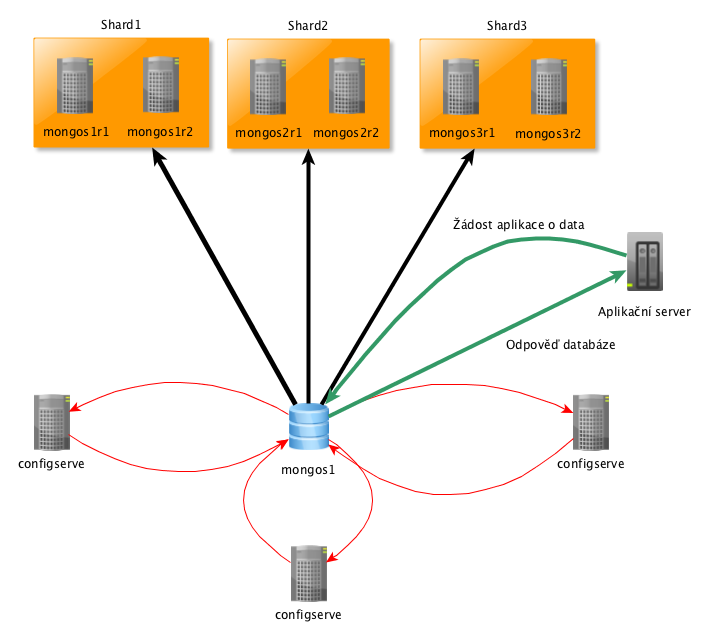
\includegraphics[scale=0.5]{obrazky/cluster-diagram}
\par\end{centering}
\caption{Schéma MongoDB databázového clusteru \label{fig:cluster-diagram}}
\end{figure}

\pagebreak
\section{Provedené testy}
Tato práce se pomocí otestování rychlosti databázových serverů pokusí rozhodnout, která z testovaných databází je vhodnější pro použití ve webové aplikaci. Vzájemně porovnávány budou relační databáze MySQL s NoSQL databází MongoDB. Porovnány budou časy zpracování základních operací s databází, tedy ukládání, editování a mazání dat. Také bude porovnán výkon těchto databází z hlediska práce s indexy. Testy indexace byly v práci zahrnuty proto, že se jedná u stávajících SQL řešení o velmi výpočetně náročnou operaci a bude zajímavé zjistit, zda-li tomu tak je i u NoSQL databází. 

Kompletní obsluhu testů zajišťuje PHP rozhraní napsané pro účely této práce, toto rozhraní má na starosti získávání náhodných dat, obsluhu databázových serverů, samotné testování a zobrazení výsledků. Samotnému testování tedy předchází ještě několik kroků.
Následující graf ukazuje jednotlivé kroky při testování a jejich podíly na celkové době běhu testu.
\begin{figure}[h]
\begin{centering}
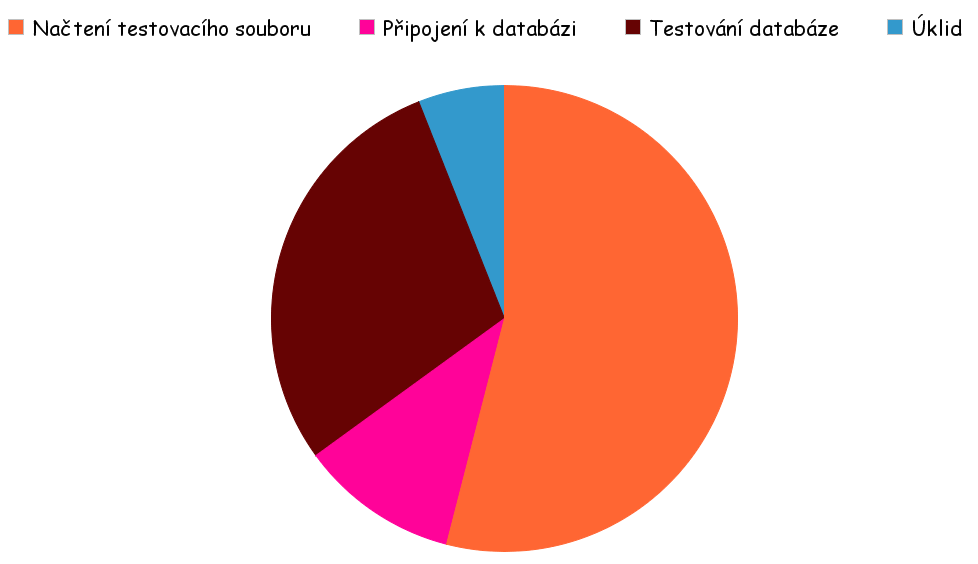
\includegraphics[scale=0.3]{obrazky/runtime-graf}
\par\end{centering}
\caption{Graf podílů jednolivých kroků při testování.\label{fig:runtimeGraph}}
\end{figure}
\FloatBarrier
Každý databázový dotaz byl před zahájením testování 5x zavolán nanečisto. Je to proto, že databázové servery provádějí optimalizace dat i za běhu a doba zpracování prvních několika dotazů bývá větší, než těch následujících.
\subsection{Ukládání dat}
Provedené testy ukládání dat simulují vytváření nových uživatelů v prostředí webové aplikace. Bylo testováno uložení 1000, 10 000 a 100 000 objektů, reprezentující fiktivní zaměstnance v organizaci. Výsledné časy jsou průměrem odezvy pěti paralelně spuštěných testů nad prázdnými databázemi.

K vkládání dat v MySQL slouží příkaz \emph{INSERT INTO} o specifické syntaxi, NoSQL databáze MongoDB používá funkci \emph{insert()}. Tato metoda přímo přijímá objekt, při testech bylo tedy možné použít rovnou objekty testovacích dat. Při testování MySQL bylo nutné vytvořit datový model, podle kterého budou data ukládaná do tabulek.
\begin{figure}[h]
\begin{centering}
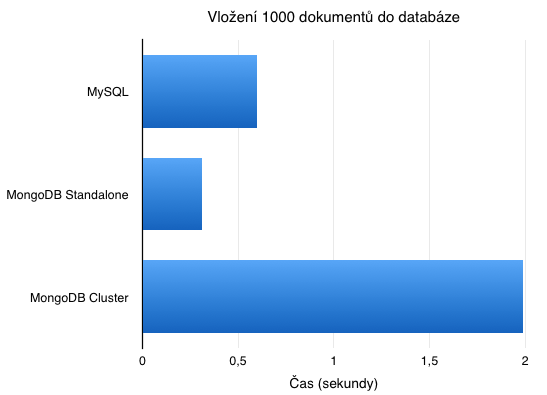
\includegraphics[scale=0.5]{obrazky/grafy/insert1000}
\par\end{centering}
\caption{Graf ilustrující dobu uložení 1000 záznamů do databáze}
\end{figure}

Jak je vidět na grafu výše, v uložení 1000 záznamů byla rychlejší databáze MongoDB. Zvládla tyto záznamy uložit za méně než půl vteřiny, naproti tomu MySQL potřebovala asi 0,7 sekundy. Cluster v testech zaostával, vzhledem k jeho virtualizované podobě nemůže konkurovat standalone variantám. Síla clusteru by se projevila až při skutečném provozu na fyzických serverech.

\begin{figure}[h]
\begin{centering}
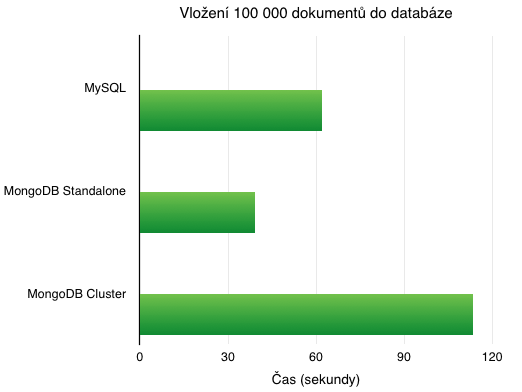
\includegraphics[scale=0.5]{obrazky/grafy/insert100k}
\par\end{centering}
\caption{Graf ilustrující dobu uložení 100 000 záznamů do databáze}
\end{figure}

Tento graf znovu dokazuje fakt, že NoSQL databáze dokáže rychleji ukládat data než MySQL. Jak je vidět, i při ukládání většího objemu dat je nejpomalejší clusterové řešení.
\subsection{Získávání dat}
Testy získávání dat si kladly za cíl simulovat situaci nalezení dané osoby v databázi a to buď přímo, za pomocí unikátního identifikátoru, nebo pomocí nějakých jeho vlastností (charakteristik). Dotazování podle unikátního identifikátoru by z principu mělo být rychlejší. V MySQL slouží k dotazování příkaz \emph{SELECT}, který nejdříve definuje tabulky a jejich sloupce, která chce získat a poté pomocí klauzule \emph{WHERE} definuje vyhledávací kritéria. MongoDB používá opačný přístup. Získávání dat probíhá pomocí funkce \emph{find()}, která v prvním parametru očekává vyhledávací kritéria. Tyto kritéria tvoří objekt, jehož atributy jsou dvojice reprezentující očekávanou hodnotu v dané vlastnosti (například \{age: 25\}). Mezi těmito atributy objektu platí logické AND. Druhým parametrem funkce find je tzv. projekce, což je objekt obsahující výčet těch atributů dotazových objektů, které mají být získány. Obě databáze tedy disponují stejnými mechanismy jen s drobnými odchylkami v syntaxi. Dotazování probíhalo nad množinou jednoho milionu záznamů.

\begin{figure}[h]
\begin{centering}
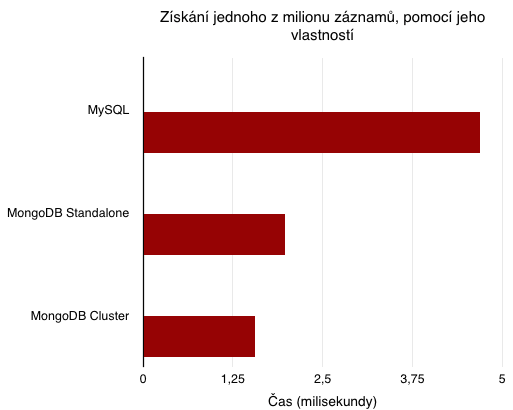
\includegraphics[scale=0.6]{obrazky/grafy/select}
\par\end{centering}
\caption{Graf ilustrující dobu nutnou pro získání jednoho záznamu pomocí jeho vlastností}
\end{figure}

\pagebreak
V oblastí získávání dat je tentokrát nejrychlejší MongoDB cluster a to i navzdory faktu, že je provozován virtuálně. Ale i varianta standalone serveru byla asi o polovinu rychlejší než MySQL. Relační databáze potřebovala k získání jednoho z milionu záznamů téměř 5 milisekund. Rozdíl mezi  získáním dat pomocí unikátního identifikátoru a pomocí vlastností daného objektu, je u NoSQL databáze zanedbatelný.  MongoDB dokáže získat záznam podle jeho klíče průměrně za 1,81 ms, zatímco podle jeho vlastností na to databáze potřebuje necelé 2 milisekundy. U relační databáze MySQL je situace odlišná. Na získání záznamu podle primárního klíče potřebuje asi 2ms, ale podle jeho vlastností téměř 5ms. Rozdíl ve rychlosti těchto dvou operací je tedy, v případě SQL databáze MySQL, značný.

\begin{lstlisting}[caption={Ukázka dotazu na osobu pomocí charakteristik v MongoDB}]
db.testData.find({
	gender:'male',
	tags:'elit',
	$or:[
		{age:{
				$gte:30
			}},
		{isActive:false}
		]
	})
\end{lstlisting}

Tento dotaz představuje ukázku složitějšího dotazování podle hodnot v daných polích. Výsledkem tohoto dotazu budou všichni muži, kteří jsou v elitní sekci a je jim buď více než 30 let, nebo již nejsou aktivní. 

Zvlášť byly testovány operace samotného dotazu na databázi (SELECT) a kompletního získání dat z databáze (SELECT + FETCH). Jednotlivé časy jsou průměrem z pěti paralelních testování. Získání dat je totiž jen jednou z částí manipulace s databází, je také nutné data načíst do struktur jazyka aplikace. Této operací se říká \emph{SELECT \& FETCH}. Testovací prostředí, použité v této práci, načítá data do PHP polí. Výsledek tohoto testu by měl být stejný jako výsledek obyčejného testu získání dat, protože samotné získání dat je nedílnou součástí tohoto testu. Z grafu níže lze potvrdit dominanci dokumentově orientované databáze MongoDB.
\begin{figure}[h]
\begin{centering}
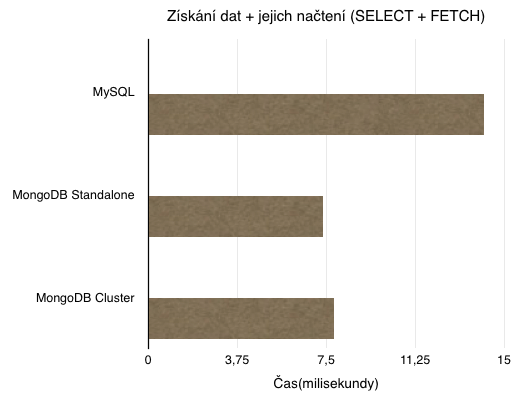
\includegraphics[scale=0.6]{obrazky/grafy/selectfetch}
\par\end{centering}
\caption{Graf ilustrující dobu nutnou pro získání jednoho záznamu pomocí jeho vlastností včetně následného načtení do struktur aplikace}
\end{figure}

\FloatBarrier
\subsection{Editace}
Další důležitou databázovou operací je editace dat, v MySQL realizovaná pomocí příkazu \emph{UPDATE}. Za tímto příkazem jsou u SQL serverů definovány změny pomocí klauzule \emph{SET}, následovanou klauzulí WHERE s vyhledávacími kritérii. NoSQL databáze obecně chápou editaci dat trochu jinak. Pohlížejí na ni jako na nahrazení jednoho objektu jiným, MongoDB k tomu nabízí funkci \emph{update}. Tato funkce očekává jako první parametr již známý objekt s vyhledávacími kritérii, druhý parametr tvoří objekt, nahrazující ten nalezený. Druhou možností je použití speciálního operátoru \emph{\$set}, který umožňuje klasickou částečnou editaci stejnou jako nabízejí SQL servery prostředníctvím příkazu \emph{UPDATE}. Tento operátor se předává v objektu v třetím parametru funkce. Zde se také pomocí operátoru \emph{\$multi} povoluje editace více dokumentů najednou.

\begin{figure}[h]
\begin{centering}
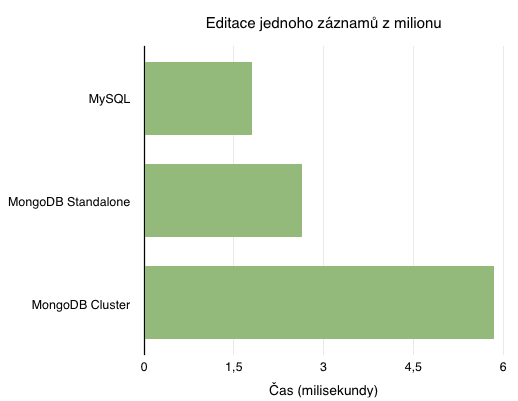
\includegraphics[scale=0.5]{obrazky/grafy/update}
\par\end{centering}
\caption{Graf ilustrující dobu nutnou pro editaci jednoho záznamu z testovací množiny}
\end{figure}
\FloatBarrier
Na grafu výše je patrné, že tentokrát byla rychlejší relační databáze MySQL, modifikace dat je také jednou z oblastí kde v tomto testování zvítězila. Je to především proto, že relační databáze MySQL je na úpravu uložených dat lépe navržena, zatímco dokumentově orientovaná databáze MongoDB s úpravami již jednou uložených objektů příliš nepočítá. Jak již bylo zmíněno, k dosažení možností editace podobné SQL příkazu \emph{UPDATE} je nutné využít operátor \emph{\$set}.

\begin{lstlisting}[caption={Ukázka editace záznamu za pomocí operátoru \$set v MongoDB}]
db.testData.update({_id:ObjectId('53e5fcaf37947b4210d69ca2')},
{$set:{index:25,isActive:true,favoriteFruit: 'apple'}})
\end{lstlisting}

\subsection{Práce s indexy}
Indexy slouží k rychlejšímu prohledávání databáze a zajišťují určité stavy sloupce napříč tabulkou. Nastavují se na parametrech objektu (MongoDB) nebo na sloupci v tabulce (MySQL). Indexy v MySQL urychlují provádění WHERE operací, poskytují záruky unikátnosti sloupce nebo umožňují fulltextově vyhledávat. Index můžeme definovat pomocí příkazu CREATE INDEX.

\begin{lstlisting}[caption={Ukázka vytvoření indexu v MySQL}]
CREATE INDEX IDX_ZAMESTNANEC_BYDLISTE
ON Zamestnanci (ulice, mesto, psc); 
\end{lstlisting}

Dokumentově orientovaná databáze MongoDB používá indexy pro urychlení přístupu k datům nebo implementaci shardingu (dělení databáze). Unikátní indexy jsou také podporovány. Ke správě indexace se v MongoDB používá metoda \emph{ensureIndex()}, která jako první přijímá objekt s definicemi indexů a jejich typů, druhým parametrem lze specifikovat typ indexu a další parametry indexace. Indexy se v MongoDB nastavují pro právě jednu kolekci.

\begin{lstlisting}[caption={Ukázka vytvoření unikátního indexu pro login v MongoDB}]
db.testData.ensureIndex({login:1},{unique:true})
\end{lstlisting}

Vzhledem ke výpočetní složitosti indexace je všeobecně doporučováno vytvářet indexy v momentě vzniku kolekce nebo tabulky, často je ale potřeba přidat nový index do kolekce,
která obsahuje data. Těch dat může být velké množství a doba vytvoření nového indexu je závislá na jejich velikosti. V rámci tohoto testování budou přidávány indexy na množinu jednoho miliónu záznamů. 

\begin{figure}[h]
\begin{centering}
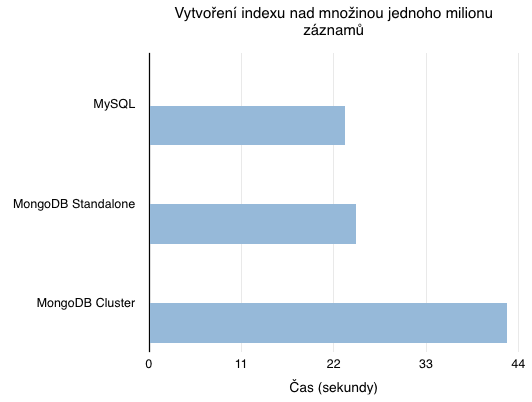
\includegraphics[scale=0.6]{obrazky/grafy/addindex}
\par\end{centering}
\caption{Graf ilustrující dobu nutnou pro vytvoření indexu nad množinou milionu záznamů}
\end{figure}
Práce s indexy představuje druhou oblast, kde v tomto testování zvýtězila relační databáze MySQL. Bylo testováno vytvoření indexu o dvou sloupcích na testovací množině jednoho miliónu záznamů. MySQL tuto úlohu zvládlo průměrně za 23,3s, NoSQL databáze MongoDB byla asi o vteřinu pomalejší a databázový cluster na tuto úlohu potřeboval téměř 44 sekund.

\subsection{Mazání dat}
Poslední operace s daty, které ještě nebyla testována, je jejich odstraňování. Mazání záznamů z databáze probíhalo na základě jejich unikátního identifikátoru, který byl náhodně vybrán z testovací množiny jednoho milionu záznamů.
\begin{figure}[h]
\begin{centering}
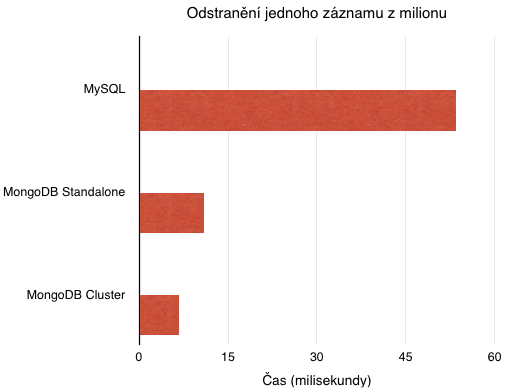
\includegraphics[scale=0.6]{obrazky/grafy/delete}
\par\end{centering}
\caption{Graf ilustrující dobu nutnou pro smazání jednoho záznamu z testovací množiny}
\end{figure}

V tomto případě úlohu nejlépe zvládl databázový cluster. Operace odstranění dat je dobrou ukázkou výhod clusteru, díky rozdělení dat na menší bloky, je v nich možné vyhledávat rychleji. Relační databáze MySQL, ukládající všechna data na jedno místo, na tuto úlohu potřebovala téměř 55 milisekund, zatímco databázový cluster jen asi 6 ms. Standalone varianta MongoDB databáze to zvládla za necelých 11 ms.

\chapter{Vyhodnocení výsledků}
Cílém této práce bylo rozhodnout, která ze dvou vytyčených databází je tou lepší pro použití ve webové aplikaci jako hlavní úložiště dat. Byly otestovány všechny operace, které jsou v moderní webové aplikaci očekávané od databázového serveru. Bohužel nelze na základě provedeného měření jednoznačně prohlásit, která z databází je pro tento účel vhodnější. Ačkoli byla NoSQL databáze MongoDB ve většině případů rychlejší než MySQL, rozdíl mezi nimy rozhodně nebyl propastný. MySQL bylo pomalejší v ukládání a získávání dat, naopak editaci dat mělo vyřešenu lépe. Úlohy získání nebo vymazání dat z velké testovací množiny miliónu záznamů zase nejrychleji zvládl MongoDB databázový cluster. Parelelní testovaní totiž nedělalo clusteru sebemenší problém. Rychlost indexace dat jednotlivých databází je velmi podobná, zde jsou rozdíly v řádu jednotek milisekund. Zajímavým faktem, který byl nameřen, je rozdíl v rychlosti těchto databází při mazání jednoho záznamu z velké množiny dat.
Relační databáze MySQL byla v tomto případě asi 5x pomalejší než MongoDB při použití standalone serveru. MongoDB cluster byl ještě rychlejší. Výsledky všech testů lze nálézt v přílohách této práce, testovací prostředí a testy samotné se nacházejí na přiloženém CD.

Velkým plusem databáze MongoDB je distribuovaný návrh. Dobře se hodí pro použití v nově vznikajících aplikacích, kde nabízí flexibilitu datových modelů a schopnost dobře reagovat na zvyšování záteže webové aplikace. Z provedených testů vyplývá, že rozdíly v rychlosti těchto databází jsou nízké, pokud si tedy vznikající webová aplikace vybere MySQL, získá veškeré schopnosti dotazovacího jazyka SQL spolu s dobrou rychlostí odezvy a dostatečným výkonem. Očekává-li se v aplikaci  velká zátěž nebo bude-li potřeba provádět operace nad velkou množinou dat, měla by webová aplikace použít některé z NoSQL řešení. Tato práce doporučuje použití dokumentově orientované databáze MongoDB při vývoji nové webové aplikace. Jedná se o moderní, výkonnou a dynamicky se rozvíjející databázi, která aplikaci nebude omezovat ani v případě velkého zájmu uživatelů. Velké odlišnosti v návrhu a datových modelech v  MongoDB však prakticky znemožňují jednoduchou migraci již existující aplikace, postavené na relačním řešení.
